\chapter{Navigeren met je horloge}

We beginnen dit kampprogramma met een klein practicum. Gebruik hiervoor een horloge met wijzerplaat (misschien heb je er een bij je, misschien kun je je smartwatch instellen om een wijzerplaat te gebruiken). Anders kun je je begeleider vragen om het horlogewerkblad.

Het doel van dit practicum is om het Noorden te bepalen, zonder kompas.

\begin{opgave}[\vinger]
    \begin{subopgave}
        Hoe laat is het nu?
    \end{subopgave}
    \begin{subopgave}
        Hoe laat is het nu -- in wintertijd?
        \begin{hint}
            In maart gingen alle klokken een uur vooruit. In oktober gaan ze een uur terug. 
        \end{hint}
        \begin{antwoord}
            Je moet een uur terug tellen van de tijd die het nu is.
        \end{antwoord}
    \end{subopgave}
\end{opgave}

Stel je horloge nu in op wintertijd, of, als je het werkblad gebruikt, teken dan eerst de juiste stand van de wijzers op de wijzerplaat - in de wintertijd. De volgende opgave voer je buiten uit, zodat je kan zien waar de zon staat.

\textbf{LET OP:} kijk nooit rechtstreeks naar de zon! Ook niet als je een zonnebril draagt. Het is beter om te kijken naar de richting van de schaduwen.

\textcolor{red}{gebruik stok/parasol als zonnewijzer?}

\begin{opgave}[\schaar]
    Zorg dat de kleine wijzer van je horloge in de richting van de zon wijst. Op je werkblad, markeer de kleinste hoek tussen de kleine wijzer en de 12. Teken vervolgens de lijn die deze hoek precies in twee\"{e}n deelt.
\end{opgave}

\begin{opgave}
    Hoe wordt deze lijn ook wel genoemd? 
    \begin{antwoord}
         Bissectrice
    \end{antwoord}
\end{opgave}

De lijn, die je zojuist getekend hebt, wijst precies naar het Zuiden. Teken nu op je werkblad de richting van het Noorden.

\begin{opgave}[\discussie]
    Terwijl je nog buiten bent, vergelijk met je groepsgenoten. Hebben jullie allemaal precies dezelfde richting gevonden voor het Zuiden? Hoe nauwkeurig denk je dat deze methode is?
\end{opgave}

\begin{opgave}
    Hoe weet je dat deze lijn precies naar het Zuiden wijst?
    \begin{antwoord}
        Om 12 uur, ofwel het middaguur, staat de Zon recht in het Zuiden. \textcolor{red}{aanvullen})
    \end{antwoord}
\end{opgave}

\begin{opgave}
    Waarom werkt deze methode minder goed als je dichter bij de evenaar bent, en beter als je dichter bij de Noordpool bent? 
    \begin{antwoord}
        Dicht bij de evenaar zijn de schaduwen korter en lijkt de zon altijd recht boven je te staan (en door de tilt van de aardas - $23.5^{\circ}$ werkt deze methode niet tussen de Kreeftskeerkring en de Steenbokskeerkring).
    \end{antwoord}
\end{opgave}

\begin{opgave}[\schaar]
    Hoe pas je deze methode aan voor de zomer? Zet je horloge terug op zomertijd en probeer of je dezelfde uitkomst krijgt.
    \begin{antwoord}
        Bepaal de kleinste hoek tussen de kleine wijzer en de 11. De bissectrice van deze hoek wijst nu recht naar het zuiden.   
    \end{antwoord}
\end{opgave}

\begin{opgave}
    Waarom werkt deze methode beter in de winter dan in de zomer? 
    \begin{antwoord}
        Je hoeft geen rekening meer te houden met zomertijd, de zon staat lager dus je kan makkelijker de richting van de schaduwen bepalen.
    \end{antwoord}
\end{opgave}

\begin{figure}
    \centering
    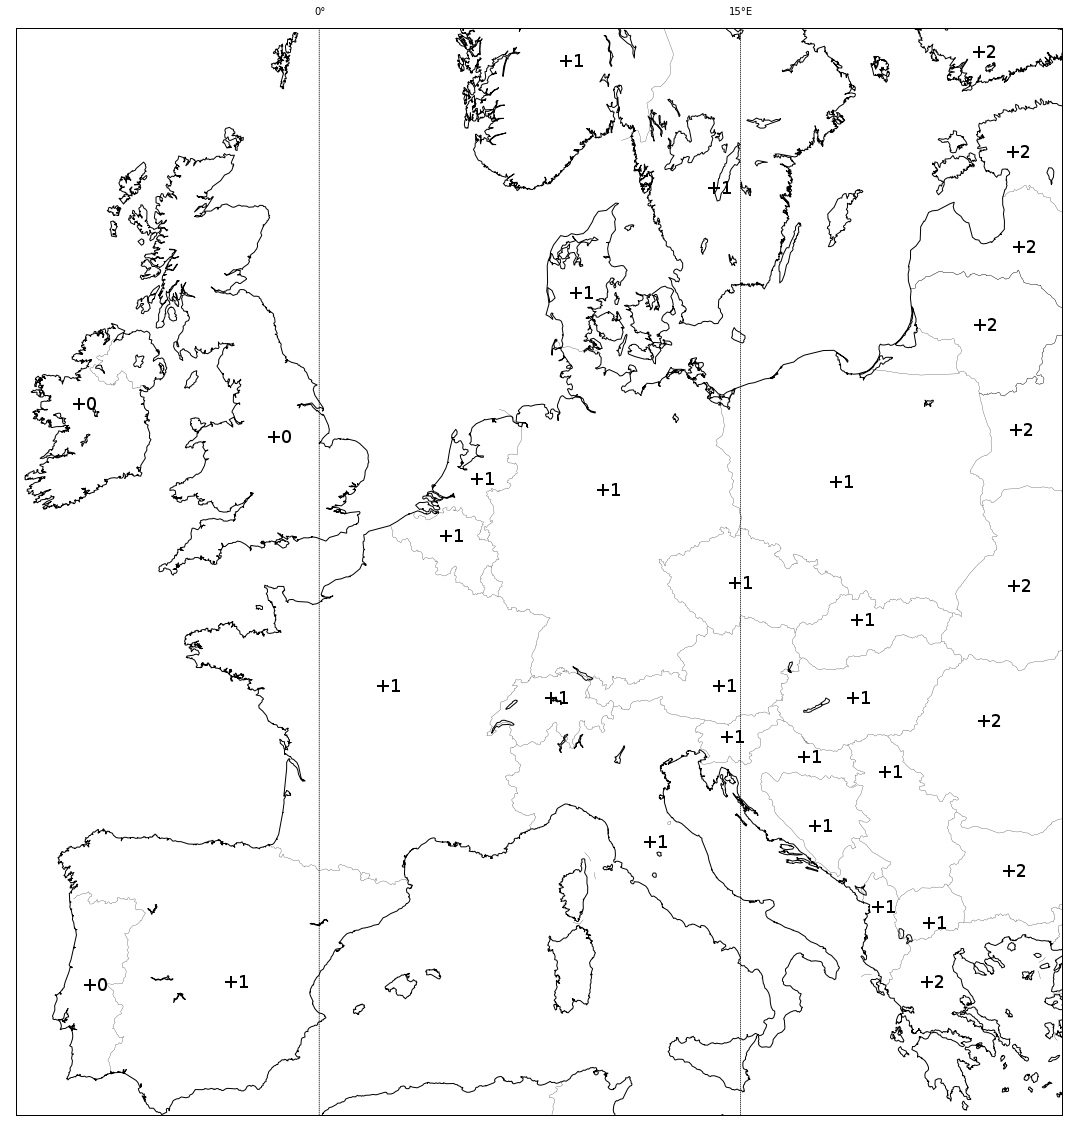
\includegraphics[width=0.7\textwidth]{europe_timezone_plus.png}
    \caption{Europa met tijdzones.}
\end{figure}

\begin{opgave}
    De offici\"ele tijd hier in Nederland is hetzelfde als in het westelijkste puntje van Spanje (dat twee tijdzones verder naar het westen ligt), maar ook hetzelfde als in het oostelijkste puntje van Polen (dat twee tijdzones verder naar het oosten ligt). Bekijk het plaatje: iedere verticale lijn geeft de theoretische grens van een tijdzone aan, maar in ieder land staat aangegeven welke tijdzone het land gebruikt. 
    \begin{subopgave}
        Wat voor problemen levert dit op?
    \end{subopgave}
    \begin{subopgave}[\ster]
        Hoe pas je de methode aan?
    \end{subopgave}
\end{opgave}

\begin{opgave}
    Hoe zou je deze methode aanpassen als je in Australi\"{e} was?
    \begin{antwoord}
        Richt de 12 van je horloge naar de zon, de bissectrice tussen de 12 en de kleine wijzer wijst nu naar het Noorden.
    \end{antwoord}
\end{opgave}

Je hebt nu gezien hoe belangrijk het is om de juiste tijd te weten als je aan het navigeren bent. Je zult later in dit programma zien dat de tijd niet alleen belangrijk is voor het bepalen van het Noorden of Zuiden met je horloge, maar ook voor het bepalen van de lengtegraad of als je een GPS apparaat gebruikt.
